\section{The control algorithm}
\subsection{}

\begin{frame}
\frametitleTC{Actuator limits}
\framesubtitleTC{}
\myPause
 \begin{itemize}[<+-| alert@+>]
 \item No physical signal can go from $-\infty$ to $\infty$.
 \item Hence control signals are invariably subject to \TC{saturation}.
 \item Modelling the relationship between a non saturated control $u_{ns}$ and the quantity $u$\\
       really exerted by an actuator with limits $(u_{min},u_{max})$ is trivial:
       \begin{displaymath}
        u(k) = \max \bigg( u_{min}, \min \big( u_{max}, u_{ns}(k) \big) \bigg).
       \end{displaymath}
 \item The point is that \TC{in the presence of a dynamic controller}, just\\
       clamping the output can make this inconsistent with the state,\\
       leading to a phenomenon called \TC{windup}. 
 \end{itemize}
\end{frame}

\begin{frame}
\frametitleTC{Windup}
\framesubtitleTC{Example with a PI}
\myPause
 \begin{columns}
  \column[T]{0.40\textwidth}
   \only<2->{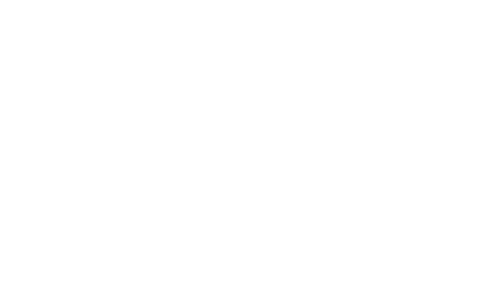
\includegraphics[height=6cm]{./Unit-06/img/example-windup-wy-u.pdf}}
  \column[T]{0.60\textwidth}
  \myPause
   \begin{itemize}[<+-| alert@+>]
   \item[1] $w$ is set to a value that cannot be obtained\\
            owing to actuator limits;
   \item[2] the really exerted $u$ stops at $u_{max}$, but as $e>0$,\\
            the computed $u_{ns}$ keeps growing due to the\\
            I action;
   \item[3] $w$ is led back to an attainable value...
   \item[4] ...but $u$ is stuck at $u_{max}$ until $u_{ns}$\\
            decreases below it, which takes\\
            some time,
   \item[5] hence $y$ remains stuck as well,\\
            and this is \TC{windup}.
   \end{itemize}
 \end{columns}
\end{frame}

\begin{frame}
\frametitleTC{Windup}
\framesubtitleTC{An important remark}
\myPause
 \begin{itemize}[<+-| alert@+>]
 \item Given its origin in a controller with I action, several texts call the phenomenon\\
       ``\underline{integral} windup''.
 \item This may be misleading, in that one may think that in the absence of I action,\\
       \TC{antiwindup} -- that we are introducing shortly -- is not necessary.
 \item WRONG. \underline{Any} \TC{dynamic} controller can generate windup: it suffices that the\\
       controller output is clamped, and the controller state is not made consistent\\
       with the clamped value.
 \item \vfill Incidentally, we just saw one possible way of realising antiwindup. 
 \end{itemize}
\end{frame}

\begin{frame}
\frametitleTC{Tracking}
\framesubtitleTC{}
\myPause
 \begin{itemize}[<+-| alert@+>]
 \item In some cases, it may be useful to constrain the controller output to track\\
       a certain signal, fed to the same controller as input.
 \item This is called the \TC{tracking} mode as opposite to the \TC{automatic} mode, in which\\
       the control law is applied normally to compute $u$.
 \item One reason for tracking can be to provide manual control, for example.
 \item In tracking mode, the state of the controller must be made consistent with the\\
       prescribed output; otherwise, when switching back to automatic mode,\\
       the first $u$ would come from the present $e$ and from the state\\
       computed the last time the controller was in automatic, in general\\
       causing an undesired transient. 
 \end{itemize}
\end{frame}

\begin{frame}
\frametitleTC{Tracking}
\framesubtitleTC{}
\myPause
 \begin{itemize}[<+-| alert@+>]
 \item Tracking is activated by a logical input generally called TS (\TC{Track Switch}):
       \begin{itemize}[<+-| alert@+>]
       \item when TS is false, $u$ is computed by the control law;
       \item when TS is true, $u$ is set equal to the value of a numeric controller input\\
             generally called TR (\TC{Track Reference}). 
        \end{itemize}
 \item We are now seeing antiwindup and tracking realised, by going through\\
       a complete PI algorithm.
 \end{itemize}
\end{frame}

\begin{frame}[fragile,label={pag:PI-complete-alg}]
\frametitleTC{A complete algorithm}
\framesubtitleTC{PI case to comment in detail}
\myPause
 {\scriptsize
 \begin{verbatim}
 e      = w-y;                   // Compute error
 up     = K*e;                   // P action needed irrespectively of the mode, see (*) below
 if not TS then                  // Automatic mode, compute I action and then u
    ui  = ui_old+K*Ts/Ti*e;
    u   = up+ui;
 else                            // Tracking mode, set u equal to TR
    u   = TR;
 end if;
 u      = max(umin,min(umax,u)); // Apply control limits
 ui_old = u-up;                  // Make state ui_old for next run consistent with u and e (*)
 \end{verbatim}
 }\myPause
 \vspace{-3mm}\begin{itemize}[<+-| alert@+>]
 \item The last line is the state management for antiwindup and tracking.
 \item This is the PI code we shall realise in Modelica: notice compactness\\
       and readability (if one knows the theory behind).
 \item If needed, porting to C, C++, fortran, java, python, whatever,\\
       is clearly straightforward. 
 \end{itemize}
\end{frame}

\begin{frame}[fragile]
\frametitleTC{A complete algorithm}
\framesubtitleTC{PID case -- study at home, ask questions next time if needed}
\myPause
 {\scriptsize
 \begin{verbatim}
 e         = w-y;
 up        = K*e;
 if not TS then
    ui     = ui_old+K*Ts/Ti*e;
    ud     = beta*ud_old+(1-beta)*K*Td/Ts*(e-e_old);
    u      = up+ui;
 else
    u      = TR;
    ud     = 0;                                      // (1) Why the arbitrary choice ud=0 here?
 end if;
 u         = max(umin,min(umax,u));
 ui_old    = u-up;
 if u>= umax or u<= umin then                        // (2) Why when u is clamped
    ud_old = 0;                                      //     ud_old for next run
 else                                                //     is set to zero
    ud_old = ud;                                     //     as well?
 end if;
 \end{verbatim}
 }\myPause
 \vspace{-6mm}\begin{itemize}[<+-| alert@+>]
 \item Suggestion for \texttt{(1)} and \texttt{(2)}: consider the relative entity of the P, I,\\
       and D actions...
 \end{itemize}
\end{frame}

